\documentclass[a4paper, 11pt, finnish]{article}
\usepackage{ucs}
\usepackage[utf8x]{inputenc}
\usepackage[T1]{fontenc}
\usepackage[finnish]{babel}
\usepackage{graphicx}
\usepackage{hyperref}

\setlength{\parindent}{0pt}
\setlength{\parskip}{1ex plus 0.5ex minus 0.2ex}

\author{Topi Talvitie}
\title{frivol: Määrittelydokumentti}

\begin{document}
\maketitle

Pistejoukon Voronoi-diagrammilla tarkoitetaan tason jakoa maksimaalisiin alueisiin siten, että kaikilla saman alueen pisteillä on sama lähin piste syötepistejoukosta. Voronoi-diagrammin alueet ovat aina monikulmioita, mahdollisesti rajoittamattomia.

\begin{figure}[h]
\centering
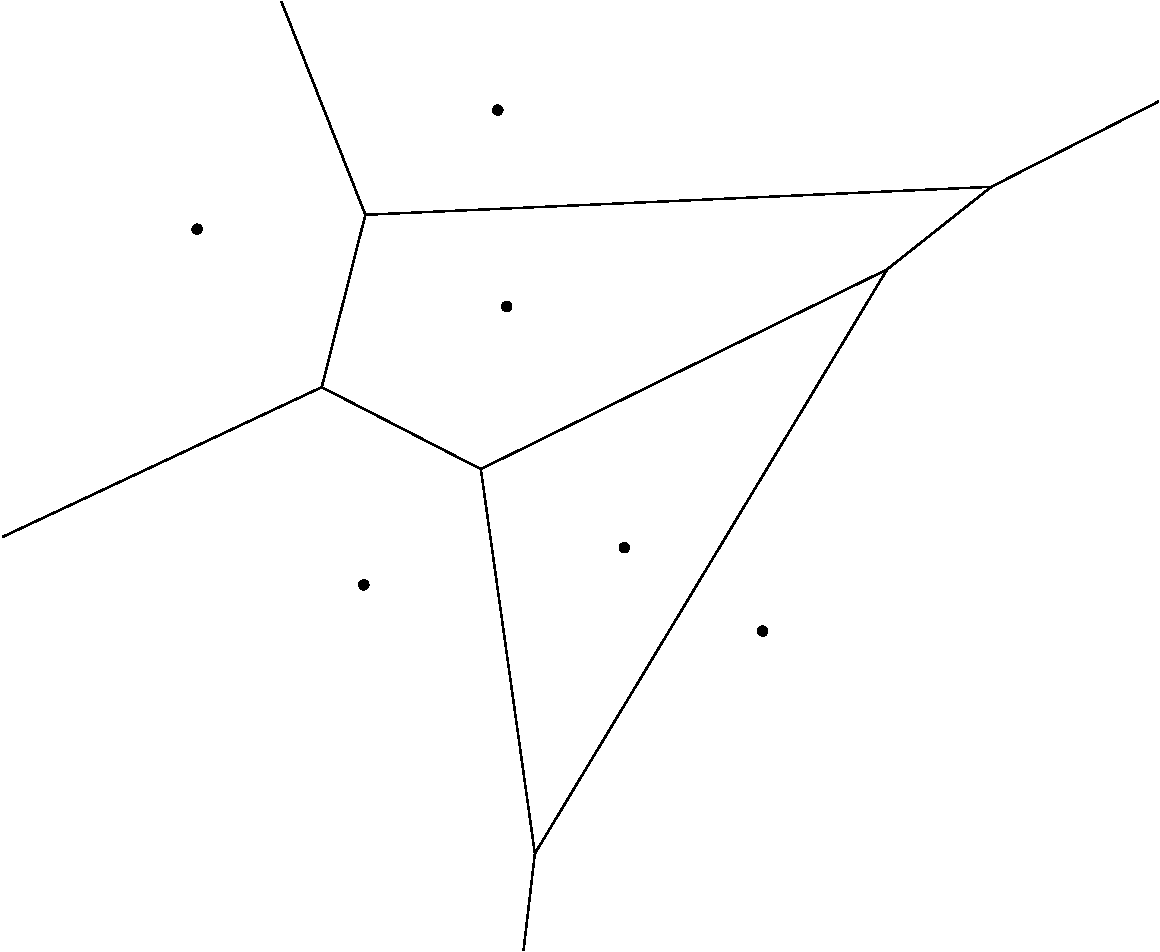
\includegraphics[height=8cm]{esim-crop}
\caption{Esimerkki pistejoukosta ja sen Voronoi-diagrammista.}
\end{figure}

Projektissa toteutetaan kirjasto annetun pistejoukon Voronoi-diagrammien laskentaan. Kirjaston nimi on \emph{frivol} eli Friendly Voronoi Diagram Library. Tämän lisäksi toteutetaan ohjelma \emph{frivoltool} joka kirjastoa käyttäen laskee annetun pistejoukon Voronoi-diagrammin ja toinen ohjelma \emph{frivoldraw}, joka osaa piirtää kuvan Voronoi-diagrammista.

\section*{Syöte ja tuloste}
Kirjaston ulkorajapinta on vain yksi funktio, joka ottaa syötteenä taulukon tason pisteitä ja palauttaa taulukon, jossa on vastaavat Voronoi-diagrammin alueet. Alue sisältää listan alueen rajoitetuista kärkipisteistä, ja mikäli alue on rajoittamaton, myös molempien rajoittamattomien sivujen suuntavektorit. Alueiden sivuihin tallennetaan lisäksi naapurimonikulmioiden indeksit.

\emph{frivoltool} on yksinkertainen ohjelma joka käärii kirjaston funktion komentorivikäyttöön sopivaksi, eli syöte saadaan ja tuloste annetaan merkkijonomuodossa.

\emph{frivoldraw} ottaa syötteen samalla tavalla kuin \emph{frivoltool}, mutta tulosteen kirjoittamisen merkkijonomuodossa sijaan se piirtää siitä kuvan, parametrien mukaan joko suoraan avattavaan ikkunaan tai kuvatiedostoon. Kuvassa näkyy pistejoukko ja Voronoi-diagrammin alueiden reunat.

\section*{Algoritmi}
\emph{frivol} laskee pistejoukon Voronoi-diagrammin käyttämällä Fortunen algoritmia, joka vie $O(n \log n)$ aikaa ja $O(n)$ tilaa, kun pisteiden lukumäärä on $n$. Fortunen algoritmissa pyyhkäisyviiva kulkee tason yli, ja samalla ylläpidetään toista pyyhkäisykäyrää joka koostuu paraabeleista jotka kasvavat muodostamaan diagrammin alueita. Pyyhkäisyviiva kohtaa matkallaan muutostapahtumia, eli uusien solmujen kohtaamisia ja vanhojen paraabelipätkien poistoja. Näitä tapahtumia on $O(n)$ kappaletta. Jokainen tapahtuman käsittely tarvitsee vain $O(1)$ kyselyä/muutosta paraabelikäyrältä, mutta vaatii sen olevan järjestetty.\cite{fortunepaperi}\cite{compgeomkirja}

Jos tapahtumien prioriteettijono toteutetaan binäärikeolla, tapahtuman lisäys ja ensimmäisen tapauksen poisto vie $O(\log n)$ aikaa, eli tapahtumien käsittely yhteensä $O(n \log n)$ aikaa. Paraabelien ketju voidaan pitää järjestettynä käyttämällä tasapainotettua binääripuuta, kuten AVL-puuta tai punamustapuuta. Koska paraabeleja on korkeintaan yksi jokaista lopputuloksen särmää kohti, eli $O(n)$, tapahtumassa käytetään $O(\log n)$ aikaa, joten tapahtumien käsittelyyn käytetään yhteensä $O(n \log n)$ aikaa. Molemmissa tietorakenteissa sekä tulosteessa\cite{fortunepaperi} on $O(n)$ alkiota, joten algoritmin muistivaativuuskin on vain $O(n)$.

Prioriteettijono voitaisiin toteuttaa samalla asymptoottisella aika- ja muistivaativuudella myös käyttäen tasapainotettua binääripuuta, jolloin tarvitsisi toteuttaa vähemmän tietorakenteita, mutta binäärikeko on vakiokertoimeltaan huomattavasti nopeampi ja lisäksi hyvin helppo toteuttaa.

\begin{thebibliography}{9}
\bibitem{fortunepaperi} S. Fortune, \emph{A sweepline algorithm for Voronoi diagrams}, Proceedings of the second annual symposium on Computational geometry, SCG '86, sivut 313-322. (\url{http://dl.acm.org/citation.cfm?id=10549}).
\bibitem{compgeomkirja} M. de Berg, M. van Kreveld, M. Overmars, O. Schwarzkopf, \emph{Computational geometry}, 2nd revised edition, Springer-Verlag 2000, sivut 151-160.
\end{thebibliography}

\end{document}
